\documentclass[oneside]{discothesis}
\usepackage[outputdir=build]{minted}
\setminted[python]{frame=lines, fontsize=\footnotesize, linenos}    

%%%%%%%%%%%%%%%%%%%%%%%%%%%%%%%%%%%%%%%%%%%%%%%%%%%%%%%%%%%%%%%%%%%%%%%%%%%%%%%%%%%%%%%%%%%%%%%%%
% DOCUMENT METADATA

\thesistype{A MEng Project Final Report} % Master's Thesis, Bachelor's Thesis, Semester Thesis, Group Project
\title{Clock and Data Recovery over Optical Links and Networks}

\author{Ammar Bin Shaqeel Ahmed}
\email{ammar.ahmed.16@ucl.ac.uk \\ 16080322}

\institute{University College London}

% Optionally, you can put in your own logo here
%logo{\includegraphics[width=0.2\columnwidth]{figures/disco_logo_faded}}

\supervisors{Dr. Georgios Zervas}
\assessor{Dr. Domaniç Lavery}

% Optionally, keywords and categories of the work can be shown (on the Abstract page)
%\keywords{Keywords go here.}
%\categories{ACM categories go here.}

\date{May, 2020}

%%%%%%%%%%%%%%%%%%%%%%%%%%%%%%%%%%%%%%%%%%%%%%%%%%%%%%%%%%%%%%%%%%%%%%%%%%%%%%%%%%%%%%%%%%%%%%%%%

\begin{document}

\frontmatter % do not remove this line
\maketitle
\cleardoublepage

\begin{acknowledgements}
 Lorem ipsum dolor sit amet, consectetur adipiscing elit. Nunc blandit tellus
 id lectus egestas, sit amet finibus diam eleifend. Nulla nulla felis,
 hendrerit vel mi ac, tempus varius libero. Proin lobortis sapien eget
 malesuada aliquet. Nulla ac eleifend velit. Suspendisse feugiat magna
 convallis, consectetur leo a, ultrices ex. Aliquam suscipit mi eu tempor
 porttitor. In facilisis eget massa ac iaculis. Sed dolor lacus, scelerisque in
 diam vitae, finibus aliquam lorem. Donec eu leo eu lorem sodales varius. Donec
 dictum mauris sed ornare porttitor. Nunc imperdiet eu elit non hendrerit. Sed
 velit lectus, lacinia sed dolor vitae, faucibus eleifend felis. Aliquam ac ex
 enim. Aliquam erat volutpat. Class aptent taciti sociosqu ad litora torquent
 per conubia nostra, per inceptos himenaeos. Pellentesque pulvinar sollicitudin
 mattis.
\end{acknowledgements}

\begin{abstract}
 Lorem ipsum dolor sit amet, consectetur adipiscing elit. Nunc blandit tellus
 id lectus egestas, sit amet finibus diam eleifend. Nulla nulla felis,
 hendrerit vel mi ac, tempus varius libero. Proin lobortis sapien eget
 malesuada aliquet. Nulla ac eleifend velit. Suspendisse feugiat magna
 convallis, consectetur leo a, ultrices ex. Aliquam suscipit mi eu tempor
 porttitor. In facilisis eget massa ac iaculis. Sed dolor lacus, scelerisque in
 diam vitae, finibus aliquam lorem. Donec eu leo eu lorem sodales varius. Donec
 dictum mauris sed ornare porttitor. Nunc imperdiet eu elit non hendrerit. Sed
 velit lectus, lacinia sed dolor vitae, faucibus eleifend felis. Aliquam ac ex
 enim. Aliquam erat volutpat. Class aptent taciti sociosqu ad litora torquent
 per conubia nostra, per inceptos himenaeos. Pellentesque pulvinar sollicitudin
 mattis.

Duis vitae malesuada tellus, malesuada tincidunt sem. Nam dapibus mattis lorem,
sagittis egestas risus ullamcorper a. Etiam finibus, libero non hendrerit
scelerisque, nisl nisi blandit lacus, id laoreet tortor turpis sit amet sapien.
Nullam non lacus ut tortor consequat auctor. Vivamus congue, massa in suscipit
imperdiet, dui neque ultricies purus, ut fermentum sapien ante vel urna. Sed at
blandit ligula. Sed non enim ante. Integer volutpat vestibulum leo, eu
malesuada diam lacinia vel. Nulla ultrices leo eu cursus feugiat. Morbi semper
nisl ex. Etiam volutpat consectetur sodales. Vestibulum facilisis dapibus enim,
ac rutrum massa blandit vehicula. Aenean nec lectus varius, congue risus at,
volutpat purus. Duis id rhoncus felis. 
\end{abstract}

\tableofcontents

\mainmatter % do not remove this line

% Start writing here
\chapter{Introduction}
Bandwidth demands in data centres have been doubling every 12-15 months. For
data centre providers to keep pace with the increased demand (at the same price
point) network switches have had to double their capacity while staying at
roughly the same cost \cite{singh2016jupiter}, and so far they have done so.
However this  seems to be coming to an end for two reasons: The first is a
predicted increase in the rate of growth of demand, due to trends like hardware
accelerated programming and dis-aggregated workloads. The second is because
electrical switches are predicted to reach a limit due to the physical limits
on pin density \cite{ballani2018bridging}.

For these reasons optical switching is being explored, as it has the potential
to overcome many of these problems. Optical switches do not require
opto-electrical (OEO) conversion, and hence the number of expensive and power
hungry transceivers required is reduced. Furthermore, as buffering is not
needed, the latency of the optical switches is much lower. Lastly, they do not
use electronics for switching, thus bypassing the aforementioned physical limit
\cite{ballani2018bridging}. 

In data centres much of the traffic that is transmitted between servers is in
the form of small data packets, with 97.8\% of packets being 576 bytes or
less~\cite{data_size}. With 100 Gb/s ports this means that switching should
take place on the order of hundreds of nanoseconds. 

When data is transmitted without a clock signal, the clock has to be
regenerated at the receiver before the data can be decoded - this is known as
clock and data recovery (CDR). The time taken for the local clock to "lock" to
the data stream, adds latency. 
In optical switches physical links are created between each
transceiver-receiver pair. Hence each time the switch is reconfigured, the CDR
must re-lock to the new link.  This means that the network throughput is
limited by the sum of the optical switching time and the CDR locking time -
which can be hundreds of nanoseconds in the worst case and tens of
nanoseconds in the best case~\cite{Chen:18}. Assuming an optical switching time
of 1 nanosecond, it is evident that the CDR locking time acts as bottleneck
that can drastically reduce the throughput~\cite{kari_phase}.

In a source synchronous system the clock is transmitted alongside the data,
removing the CDR locking time. This would remove the bottleneck, theoretically
increasing the throughput.


\chapter{Theoretical Basis}

\section{Background Theory}%
\label{sec:background_theory}
Here we go deeper into the theory of certain elements of the system.

\subsubsection{Bang-Bang CDR}%
\label{ssub:clock_and_data_recovery}
Commonly a serial data stream is sent over a channel without a clock signal.
Clock and Data Recovery (CDR) is the process of extracting timing information
from a serial data stream, then using it to decode the received data stream.  A
CDR circuit has two primary functions. The first is to extract a clock based on
the input data, and the second is to resample the data. 

To extract the clock from the data, a local clock is generated, then is adjusted
as "early" or "late" when compared with the incoming data
signal \cite{sun1989analog}.  We can think of this as a control system, as
shown in Figure~\ref{fig:cdr_basic}.

\begin{figure}[ht]
    \centering
    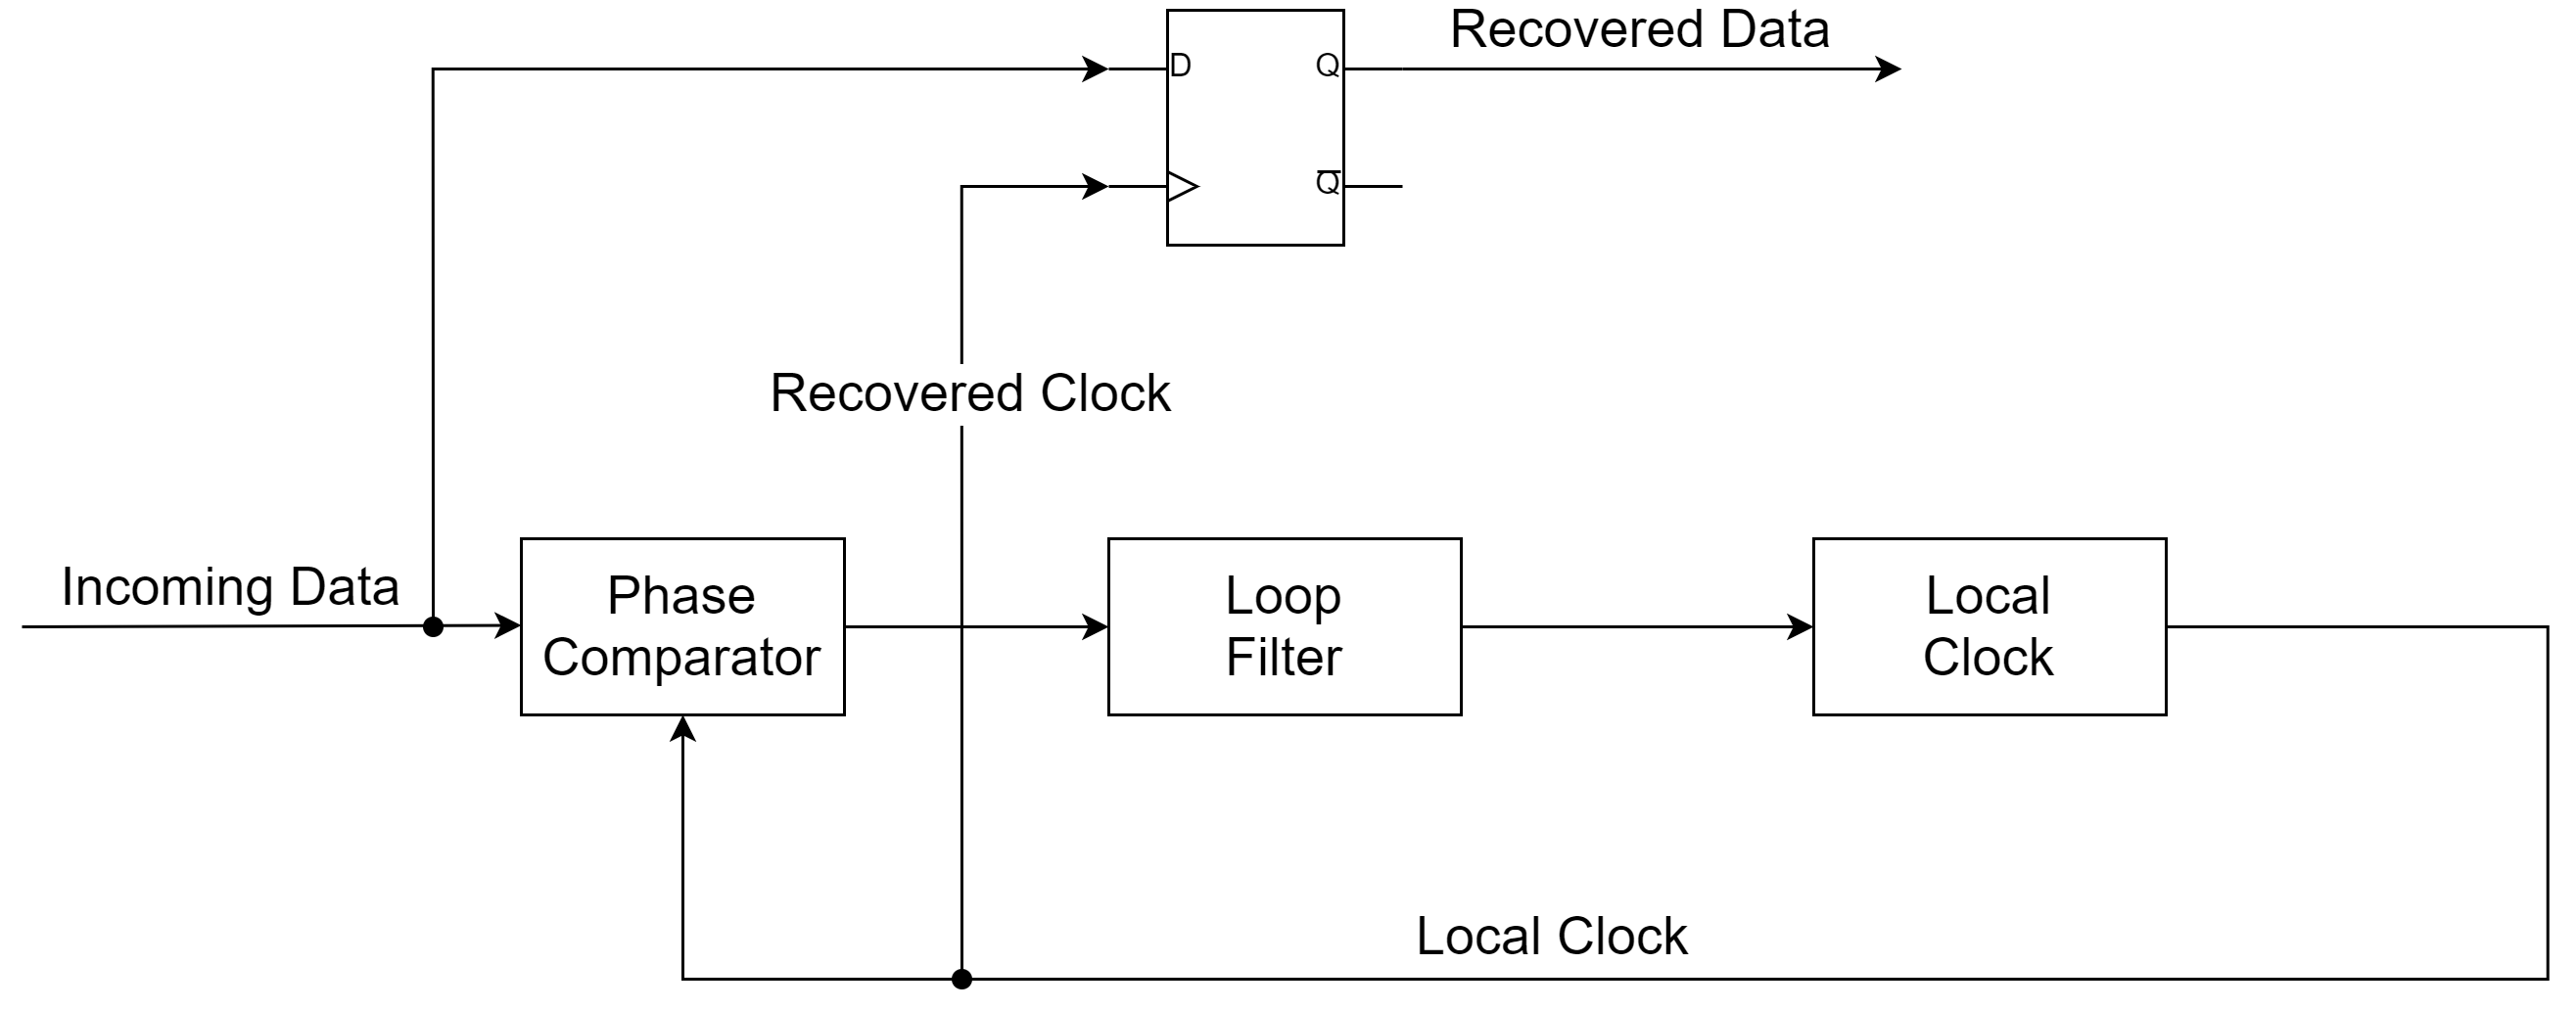
\includegraphics[width=1\linewidth]{img/cdr_basic.png}
    \caption{Basic CDR design}%
    \label{fig:cdr_basic}
\end{figure}

Phase detectors can be divided into two types, linear (where the output has a
linear relationship to the input) and binary or bang-bang phase detectors (where the output
is either positive or negative). Binary phase detectors are more commonly used
in digital CDR circuits~\cite{ZHANG2015163}. An example of one is the
Alexander detector \cite{alexander1975clock} which gives out a high D0+ and a low D0- if the
clock lags and vice-versa if the clock leads, as shown in
Figure~\ref{fig:bang_bang}.

\begin{figure}[ht]
    \centering
    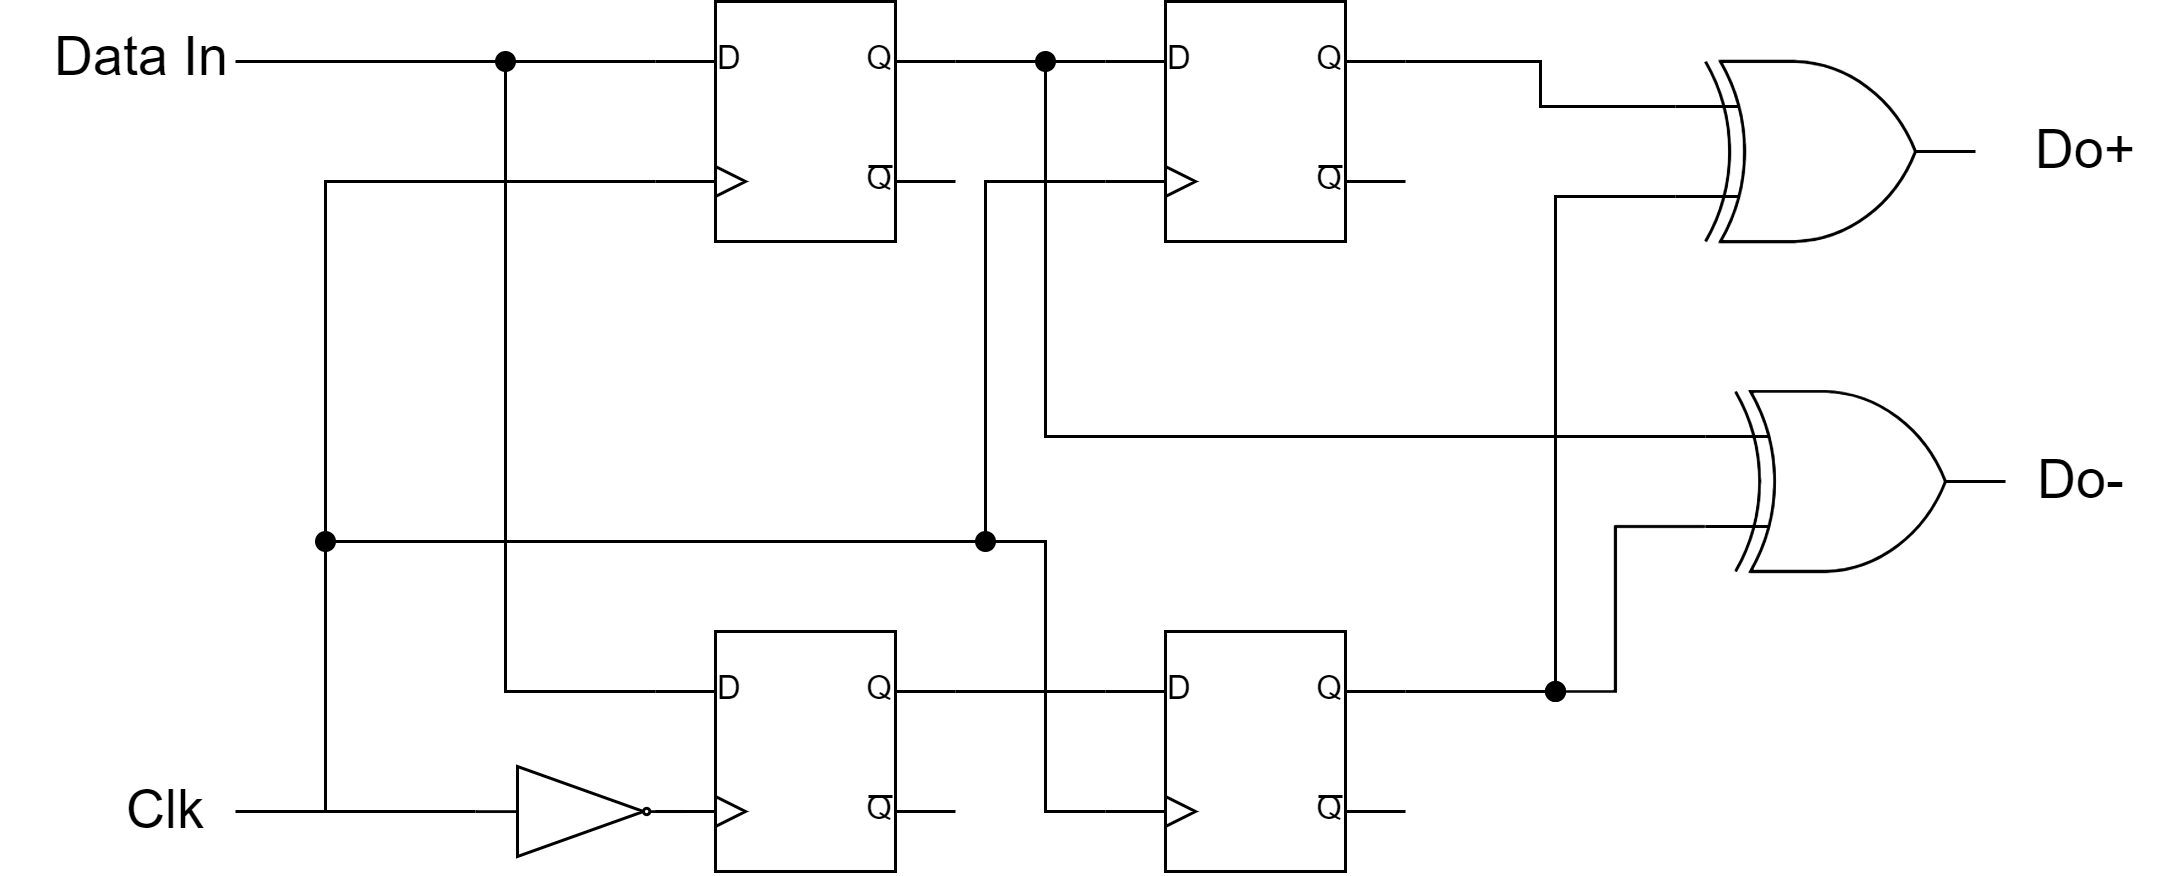
\includegraphics[width=0.8\linewidth]{img/bang_bang.png}
    \caption{Alexander Phase Detector}%
    \label{fig:bang_bang}
\end{figure}

\subsubsection{Pseudorandom Binary Sequence}%
\label{ssub:prbs_generation}
A pseudorandom binary sequence (PRBS) is a sequence of bits that appears to be
random. However as it is generated using a deterministic algorithim, it can be
replicated if the inital conditions are the same.

A common practical implementation of PRBS generation uses linear-feedback shift registers.  As an
example, a PRBS-4 sequence could be generated by using a 4 bit register. We
seed the register with a non-zero number, then tap two bits of the register as
an input. We then shift the contents of the register, taking the last bit as an
output and the new bit as an input, as illustrated in
Figure~\ref{fig:img/shift_reg}.

\begin{figure}[ht]
    \centering
    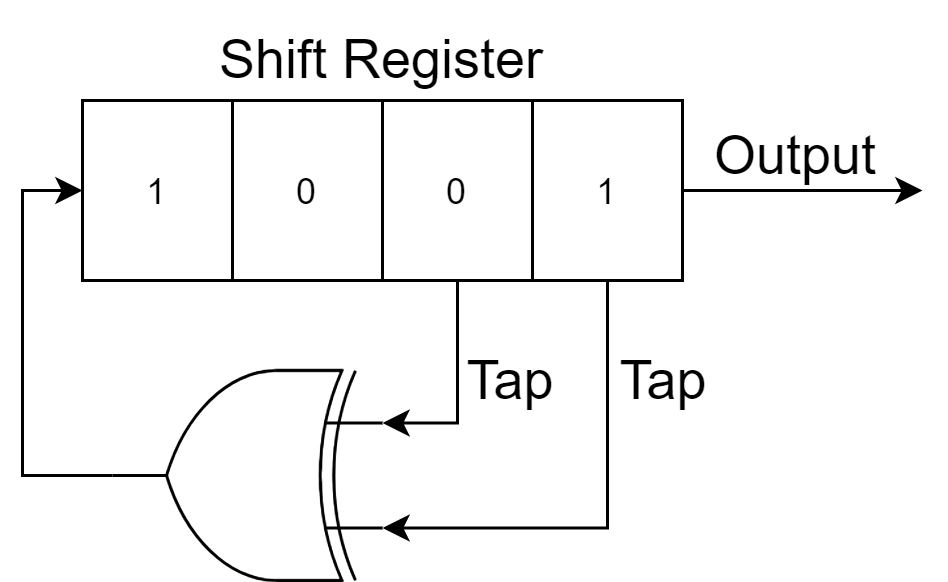
\includegraphics[width=0.4\linewidth]{img/shift_reg.png}
    \caption{Shift Register Implementation}%
    \label{fig:img/shift_reg}
\end{figure}

The full operation can be seen in Table~\ref{tab:shift_reg}. As 0000 cannot
appear (the value of the register would never change) we see that for a register of size N, the
bitsequence is $2^N - 1$ bits long. 
\begin{table}[ht]
    \centering
    \begin{tabular}{|c|c|c c c c|c|}
    \hline
    Cycle & Input & \multicolumn{4}{|c|}{Shift Register} & Output \\
    \hline
     0  & 1 & 1 & 0 & 0 & 1 & 1 \\
     1  & 0 & 1 & 1 & 0 & 0 & 0 \\
     2  & 1 & 0 & 1 & 1 & 0 & 0 \\
     3  & 0 & 1 & 0 & 1 & 1 & 1 \\
     4  & 1 & 0 & 1 & 0 & 1 & 1 \\
     5  & 1 & 1 & 0 & 1 & 0 & 0 \\
     6  & 1 & 1 & 1 & 0 & 1 & 1 \\
     7  & 1 & 1 & 1 & 1 & 0 & 0 \\
     8  & 0 & 1 & 1 & 1 & 1 & 1 \\
     9  & 0 & 0 & 1 & 1 & 1 & 1 \\
     10 & 0 & 0 & 0 & 1 & 1 & 1 \\
     11 & 1 & 0 & 0 & 0 & 1 & 1 \\
     12 & 0 & 1 & 0 & 0 & 0 & 0 \\
     13 & 0 & 0 & 1 & 0 & 0 & 0 \\
     14 &   & 0 & 0 & 1 & 0 & 0 \\
    \hline
    \end{tabular}
    \caption{Shift Register Operation}
    \label{tab:shift_reg}
\end{table}

\subsubsection{Semiconductor Optical Amplifier}%
\label{ssub:semiconductor_optical_amplifier}
A Semiconductor Optical Amplifier (SOA) is 



\subsubsection{Source Synchronous System}%
\label{ssub:source_synchronous_system}
In a source synchronous system a clock signal is provided alongside the data
signal, as shown in Figure~\ref{fig:source_sync}. This has the advantage of not
needing a CDR circuit. Furthermore as both the clock and the data come from the
same device any jitter will be similar across both signals and can likely be
ignored \cite{ragab2011receiver}.   A downside is that there will be crossing
of clock domains at the reciever as the transmitted clock will not be
synchronous with the clock domain of the receiving device.
\begin{figure}[ht]
    \centering
    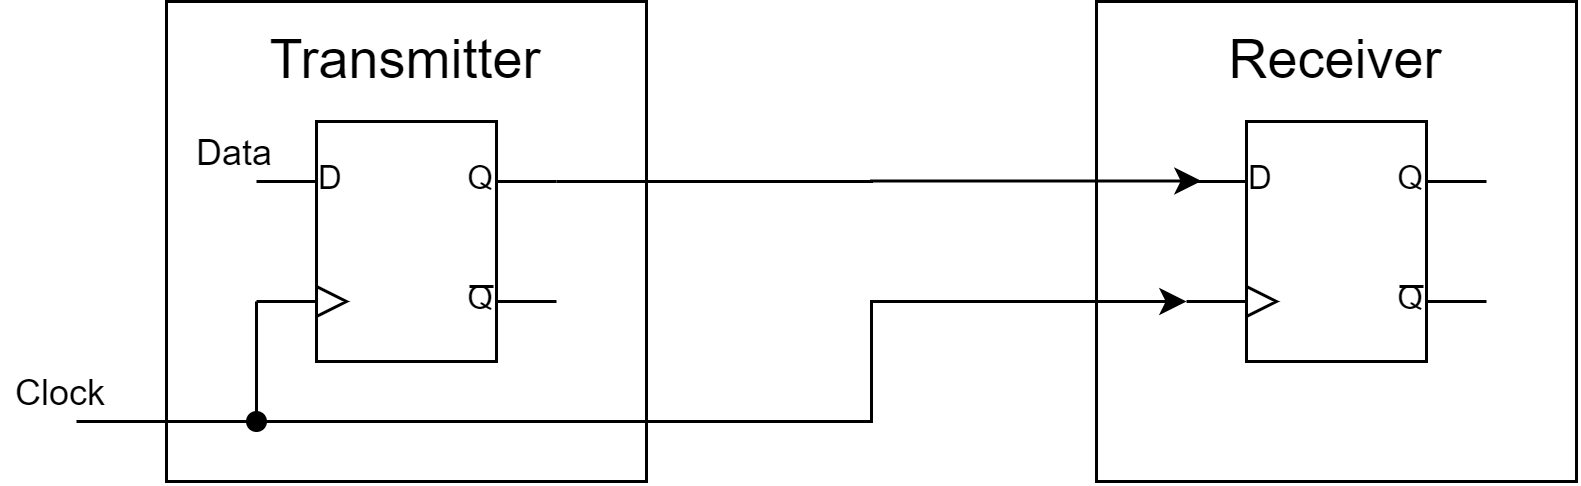
\includegraphics[width=0.8\linewidth]{img/source_sync.png}
    \caption{Source Synchronous System}%
    \label{fig:source_sync}
\end{figure}

\section{Literature Review}%
\label{sec:literature_review}

\noindent \cite{kari_phase} outlines how CDR circuits are a limiting factor in
optical switching and proposes a method of phase caching to overcome this.
Here the phase of the local clock in relation to the data is cached.  The PRBS
data is pregenerated (written to memory) and is sent in short bursts with a
known sequence at the end. When the data arrives it is then written to memory
and then processed.  The phase caching improved locking time on switching by 12
times.

\noindent In \cite{serrano2013white}, \cite{moreira2010digital}, and
\cite{moreira2009white}, the white rabbit project is discussed. A white rabbit
system provides sub-nanosecond synchronisation accuracy. To achieve this,
accurate measurements of the link delay between the nodes of the network must
be calculated.  While instructive, the method is not directly applicable to the
project, as in a White Rabbit system, all the nodes are locked to the same
frequency. Hence the link delay can be calculated by having a node receive a
clock signal from another node, then return the same signal. The link delay can
then be calculated by comparing the phase offset of the two signals.

\noindent \cite{williams2016source} described an optical source synchronous
system. It describes how choosing the correct wavelength for the clock can
minimise the modal cross-talk. Furthermore, in conjunction with
\cite{ragab2011receiver} it describes how source synchronous systems are able
to track correlated jitter between clock and data channels, and how system
performance can be degraded by channel slew between clock and data channels.\\
\cite{williams2019reconfiguration} further explored reducing the modal
crosstalk by proposing an architecture with re-configurable clock and data
paths, thus allowing the user to chose the optimal lane for the sensitive clock
for each photonic interconnect. This may not be needed however, as each
transmitter should have a fixed data characteristic.

\noindent \cite{chen2017optimization} and \cite{fixed_latency} describe fixed
latency links. In the event we were unable to bypass the CDR, it may be
possible to organise the system to have a fixed latency, then force the CDR to
the appropriate fixed phase. Thus the circuit could thus have a much reduced
CDR lock time.

\noindent \cite{dru_guide}, \cite{nidru} describe an Xilinx intellectual
property that allows the high speed serial transceivers to be used at much
lower data rates. This was initially of interest because it would have been
easier to demonstrate a working system with lower data rates. However as this
is an extra IP used in conjunction with the transceivers it did not turn out to
be useful for the project. 

\noindent \cite{mendes_transceiver} this presentation describes a system where
the phase of a transceiver on Xilinx board is kept stable over resets. While
this was done on the transmitter side it shows that fixing the phase of the
transceiver is possible.


\chapter{Proposed System and Objectives}

\section{Proposed System Overview}%
\label{sec:system_overview}
To demonstrate the efficacy of a source synchronous system we propose a single
pseudorandom binary sequence (PRBS) source that optically transmits over two
channels to a single receiver. If transmission is alternated the effect is that
the receiver would receiver bursts of data from two different channels. If the
full PRBS sequence is received then the system would be working correctly.\\ An
overview of the system is shown in Figure~\ref{fig:overview}. 

\begin{figure}[h]
    \centering
    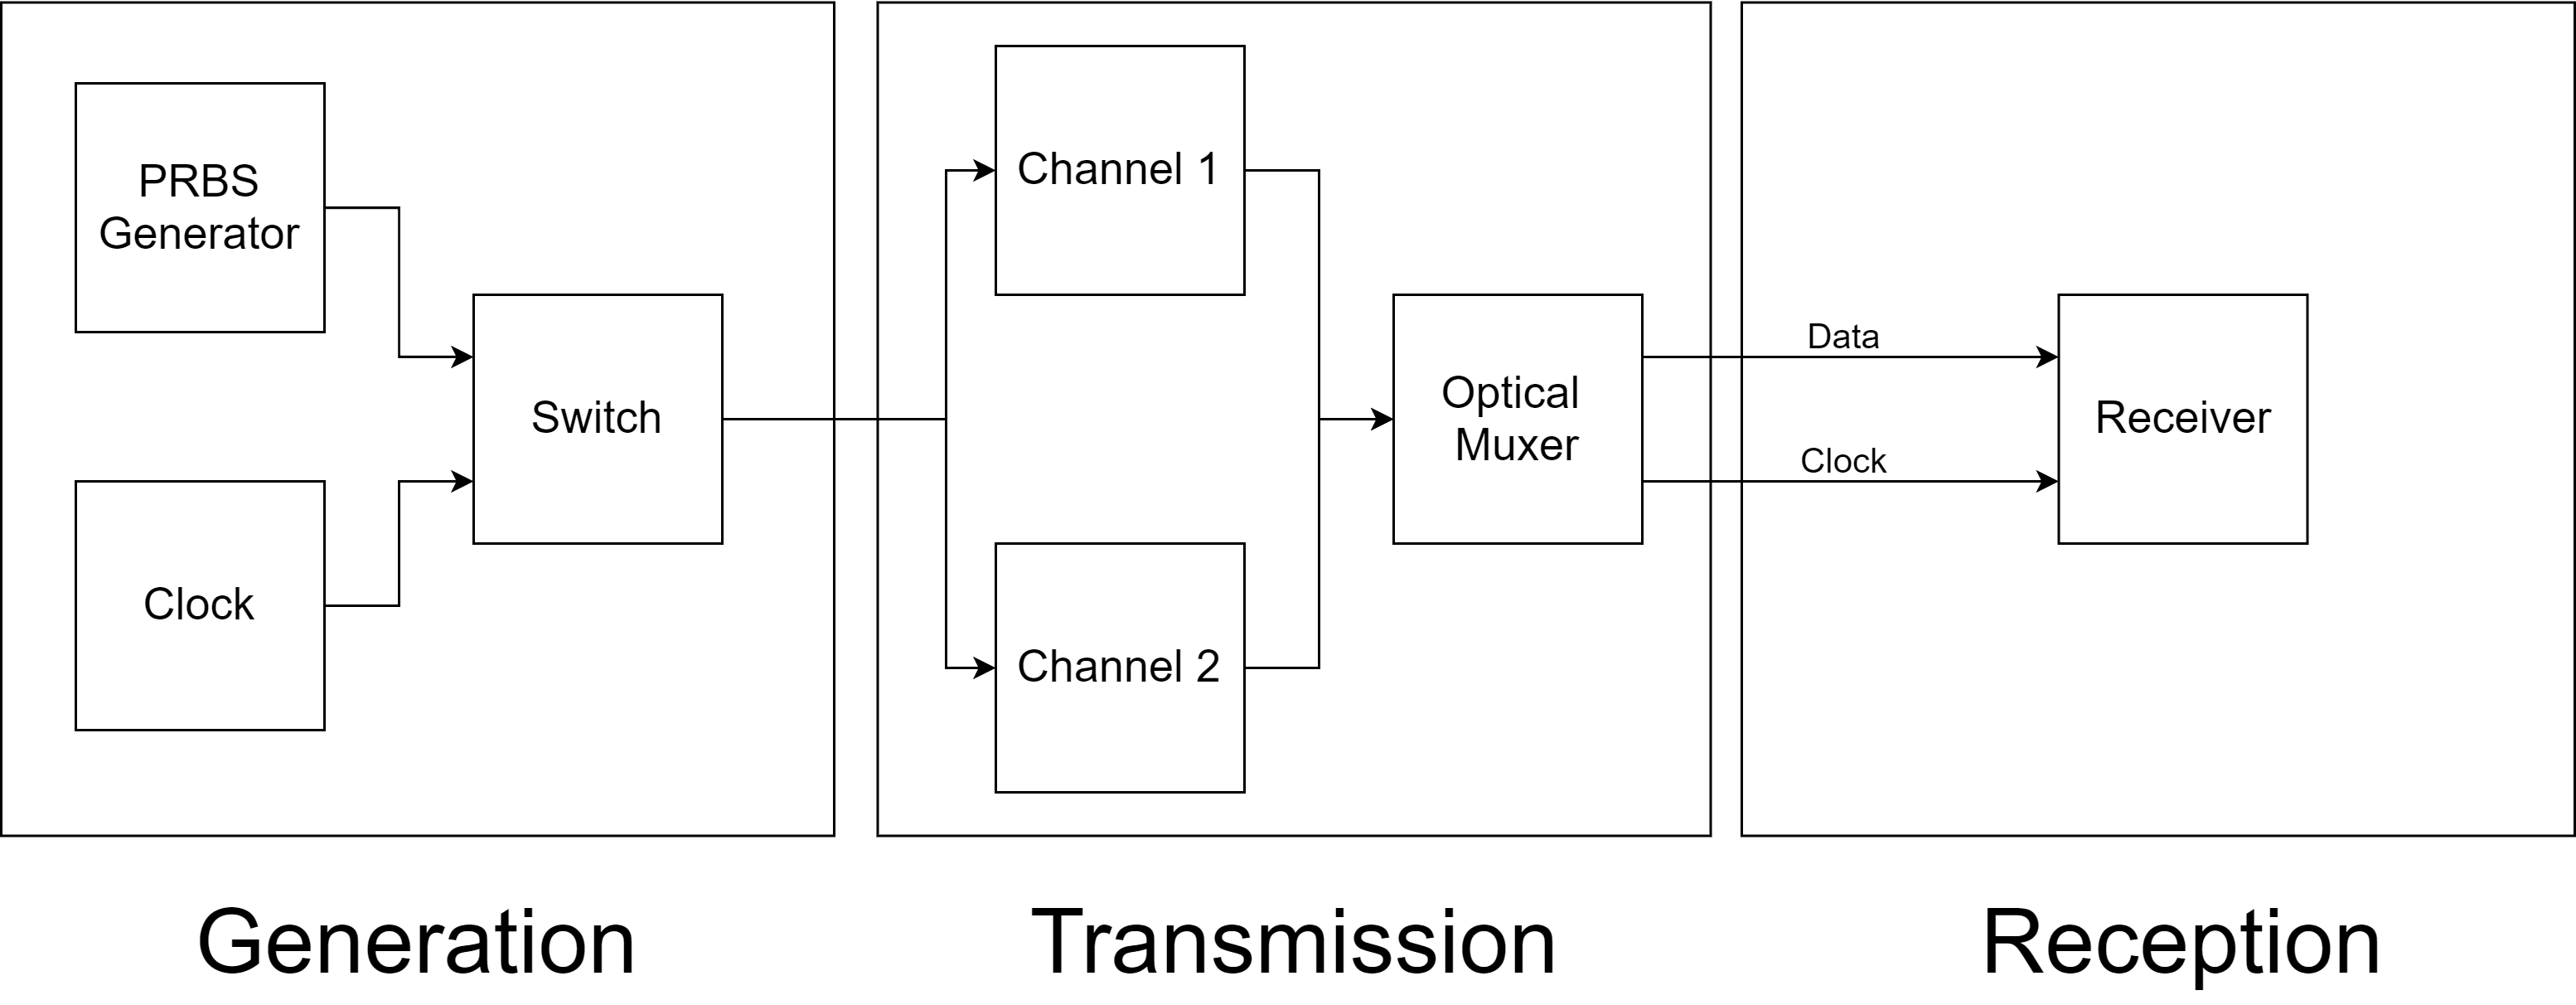
\includegraphics[width=1\linewidth]{img/overview.png}
    \caption{Overview of System}%
    \label{fig:overview}
\end{figure}

\section{Objectives}%
\label{sec:objectives}
The overall objective is to develop a successful burst source-synchronous
communication system for comparison with a system that uses a CDR.
\noindent
Overall we can break down the project to the following sub-objectives: 
\begin{itemize}
    \item Burst mode PRBS transmission over two channels alongside clock
    \item Optical transmission over two channels, then muxing the two channels together
    \item Source-synchronous reception of PRBS data 
\end{itemize}

\chapter{Implementation and Results}
In this section we cover the implementation of the project and the results.
As outlined in the Objectives section we can divide the tasks into three main
parts: transmission, optical conversion ,and reception. 
In this project we looked at using a FPGA board for the generation and
reception of the PRBS data.  Hence the overall design is of a board in a
loopback configuration as shown in Figure~\ref{fig:loopback}.

\begin{figure}[ht]
    \centering
    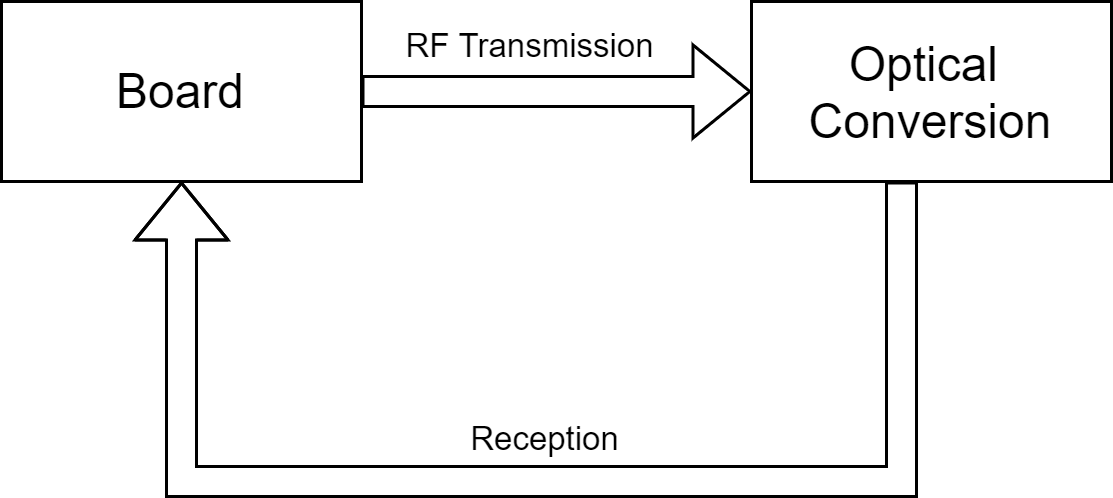
\includegraphics[width=0.5\linewidth]{img/loopback.png}
    \caption{Loopback Configuration}%
    \label{fig:loopback}
\end{figure}

\section{Transmission and Reception}%
\label{sec:transmission_and_reception}




\subsection{Hardware}%
\label{sub:hardware}
To generate and receive PRBS data the VCU118 board was used. The transmission
and reception of the data was handled by the onboard high-speed parallel to
serial GTY transceivers in conjuction with a Si5345 external clock. To connect
with the transceiver the HiTechGLobal FMC-MSMP module was used.
\begin{figure}[ht]
    \centering
    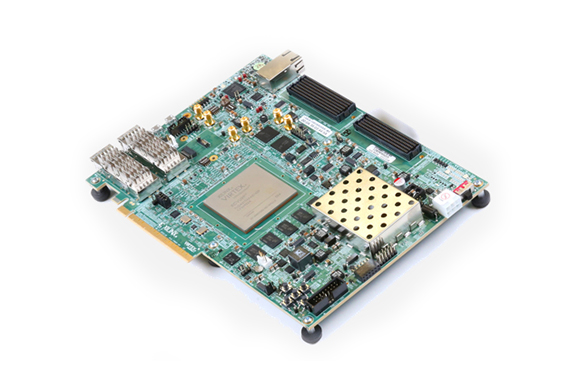
\includegraphics[width=0.5\linewidth]{img/board.jpg}
    \caption{VCU118 Board}%
    \label{fig:board}
\end{figure}

\begin{figure}[ht]
    \centering

    \begin{minipage}[b]{0.6\textwidth}
        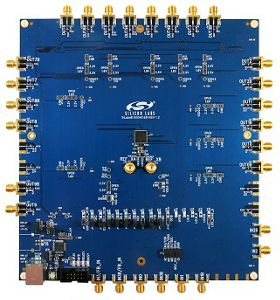
\includegraphics[width=0.8\linewidth]{img/clock.jpg}
        \caption{Si5345 Clock}%
        \label{fig:clock}
    \end{minipage}
    \hfill
    \begin{minipage}[b]{0.3\textwidth}
        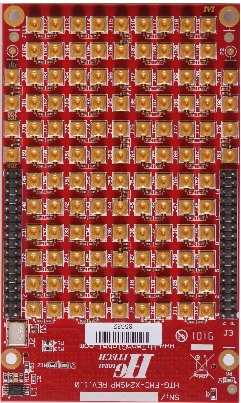
\includegraphics[width=0.8\linewidth]{img/fmc.png}
        \caption{FMC-MSMP module}%
        \label{fig:fmc}
    \end{minipage}

\end{figure}

\subsection{Transceiver Setup}%
\label{sub:transceiver_setup}
Most of the project took place using the transceivers in a simple RF loopback
configuration (no optical transmission).

The setup of the transceivers followed the example design outlined in the user
guide to the transceivers \cite{wizard_guide}. Places where choices were made
(as the example design is not specific to a particular board) or the
design was deviated from are outlined below. 

\subsubsection{Selection of Quads}%
\label{ssub:selection_of_quads}
The GTY transceivers in the VCU118 are grouped into four channels or quads.
Seven GTY quads on the left side of the device and six GTY quads on the right
side of the device.
There are 52 transceivers on VCU118 board, in total.
\begin{itemize}
    \item Four of the GTY transceivers are wired to Samtec Firefly Module Connector 
    \item Four of the GTY transceivers are wired to QSFP1 module connector 
    \item Four of the GTY transceivers are wired to QSFP2 module connector 
    \item Sixteen of the GTY transceivers are wired to the PCIe 16-lane edge connector
    \item Twenty-four of the GTY transceivers are wired to FMC+ HSPC connector
\end{itemize}

As we were using a FMC-HSMP module to connect to the transceivers, we were limited to the transceivers wired
to the FMC+ HSPC connector.
Furthermore only certain quads can be driven through an external clock.
As such we chose Quad 120 and Quad 122 as the quads for testing.

There are also limitations to the number of quads that can be driven with an
external clock while still meeting jitter requirments, but as we are only
driving two transmitters, it was not an issue.



\subsubsection{Pin Configuration}%
\label{ssub:pin_configuration}
It was also necessary to map the pins from the pins on the board to those on
the FMC-MSMP module. This was done as in Table~\ref{tab:pinout}.
As two transceivers were used, we mapped out the pins for clocks, transmitters,
and recievers of both.

\noindent For a full pinout diagram refer to the user guide of the board
\cite{vcu118_guide}. 

\begin{table}[ht]
    \centering
    \hspace*{-3.5cm}\begin{tabular}{|c|c|c|c|c|c|}
        \hline
        Function & Channel & Net Name & FPGA PIN & Connected Pin & FMC+ Pin \\
        \hline
        clk\_p & GTYE4\_COMMON\_X0Y1  & FMCP\_HSPC\_GBTCLK5\_M2C\_P & AN40 & Z20 & J106 \\
        clk\_n & GTYE4\_COMMON\_X0Y1  & FMCP\_HSPC\_GBTCLK5\_M2C\_N & AN41 & Z21 & J115 \\
        tx\_p  & GTYE4\_CHANNEL\_X0Y4 & FMCP\_HSPC\_DP20\_C2M\_P    & BD42 & Z8  & J117 \\
        tx\_n  & GTYE4\_CHANNEL\_X0Y4 & FMCP\_HSPC\_DP20\_C2M\_N    & BD43 & Z9  & J116 \\
        rx\_p  & GTYE4\_CHANNEL\_X0Y4 & FMCP\_HSPC\_DP20\_M2C\_P    & BC45 & M14 & J55  \\
        rx\_n  & GTYE4\_CHANNEL\_X0Y4 & FMCP\_HSPC\_DP20\_M2C\_N    & BC46 & M15 & J54  \\
        \hline
        clk\_p & GTYE4\_COMMON\_X0Y3  & GBTCLK2\_M2C\_P             & AF38 & L12 & J21  \\
        clk\_n & GTYE4\_COMMON\_X0Y3  & GBTCLK2\_M2C\_N             & AF39 & L13 & J20  \\
        tx\_p  & GTYE4\_CHANNEL\_X0Y8 & DP0\_C2M\_P                 & AT42 & C2  & J77  \\
        tx\_n  & GTYE4\_CHANNEL\_X0Y8 & DP0\_C2M\_N                 & AT43 & C3  & J78  \\
        rx\_p  & GTYE4\_CHANNEL\_X0Y8 & DP0\_M2C\_P                 & AR45 & C6  & J100 \\
        rx\_n  & GTYE4\_CHANNEL\_X0Y8 & DP0\_M2C\_N                 & AR46 & C7  & J99  \\
        \hline
    \end{tabular}
    \caption{Transceiver Pin Out}
    \label{tab:pinout}
\end{table}


\subsubsection{Transceiver Configuration}%
\label{ssub:transceiver_configuration}
The transceivers were programmed to run at a standard rate of 10GB/s, with a
reference clock taken from the external Si5345 clock which was configured to
run at 156.25 MHz with a format of 2.5 V LVDS.
The free-running clock (used to drive resets) was driven at 125 MHz, sourced
from the onboard 300 MHz system clock.  The reset functions were bound to the
physical push buttons BE23 and BB24.  Status indicators (Link Up and Link Down)
were bound to LED1 and LED0 respectively. 

At the current stage there was no encoding in the setup as we were trying to
troubleshoot an issue with the PRBS checking module. However if running the
system for a long period of time, encoding would be necessary to ensure the CDR
remained locked.
The full details of the setup can be found in
Appendix~\ref{cha:transceiver_settings}.


\subsection{Transmitter}%
\label{sub:transmitter}
In Figure~\ref{fig:transmitter_block} we see a block diagram of the transmitter
(TX) of the transceiver. Parallel data flows into the TX interface,
and is serialised, then finally flows out of the transmitter as high-speed
serial data.

\begin{figure}[ht]
    \centering
    \hspace*{-1cm}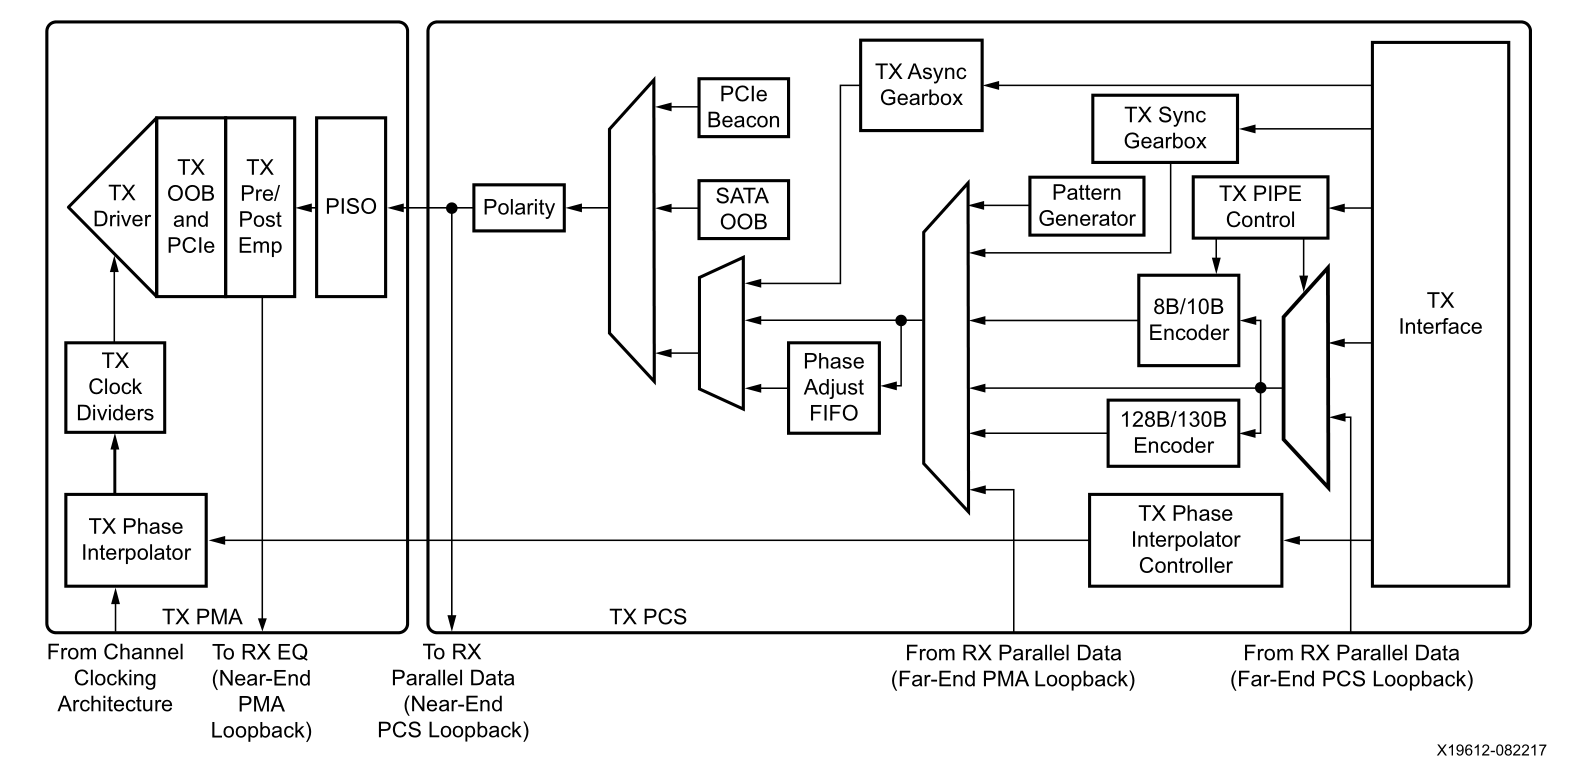
\includegraphics[width=1.2\linewidth]{img/transmitter_block.png}
    \caption{Transmitter Block Diagram~\cite{GTY_guide} }%
    \label{fig:transmitter_block}
\end{figure}

We looked to modify the functionality of a basic implementation of the
transmitter. In the basic implementation a PRBS generator that generates a
sequence through shift registers (as outlined in
Section~\ref{ssub:prbs_generation}) is is fed to the transmitter interface. 

The PRBS module was mainly unchanged from the default with some minor
adjustments.  There were two variations of the PRBS generation module that were
developed.

\subsubsection{Burst Mode over Single Channel}%
\label{ssub:burst_mode_over_single_channel}
Here we modified the PRBS generation module and set it to output zeros if the
enable command was not asserted.  In combination we added a register
inside the wrapper, which on overflow toggles the enable flag. This has the
effect of causing the PRBS module to output a sequence interspersed with zeros.

A testbench where both the unmodified PRBS generator and burst PRBS generator
are compared is shown in in Figure~\ref{fig:burst_mode_start}.  We see the
burst generator correctly generating the expected PRBS sequence interspersed
with zeros. We note also that the full sequence is transmitted in burst mode (no
data is lost).

\begin{figure}[ht]
    \centering
    \hspace*{-3cm}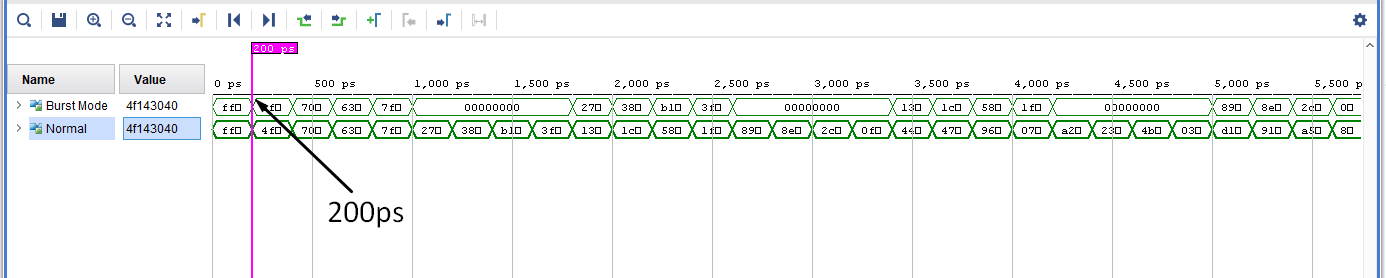
\includegraphics[width=1.5\linewidth]{img/burst_mode_1.png}
    \caption{Single Burst Mode Behaviour}%
    \label{fig:burst_mode_start}
\end{figure}

Comparing Figure~\ref{fig:normal_mode_recur} and
Figure~\ref{fig:burst_mode_recur} we see that the recurrence time (in this
testbench we use PRBS7, as it is a short sequence) for the normal sequence as
compared with the burst mode sequence is about half. This makes sense as the
burst mode sequence is operating on a duty cycle of 50\% and hence should take
roughly double the time to recur.

\begin{figure}[ht]
    \centering
    \hspace*{-3cm}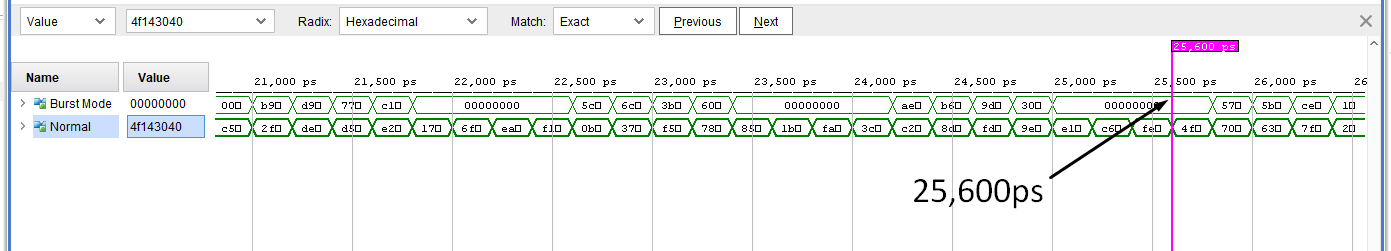
\includegraphics[width=1.5\linewidth]{img/burst_mode_2.png}
    \caption{Normal Mode Recur Time}%
    \label{fig:normal_mode_recur}
\end{figure}

\begin{figure}[ht]
    \centering
    \hspace*{-3cm}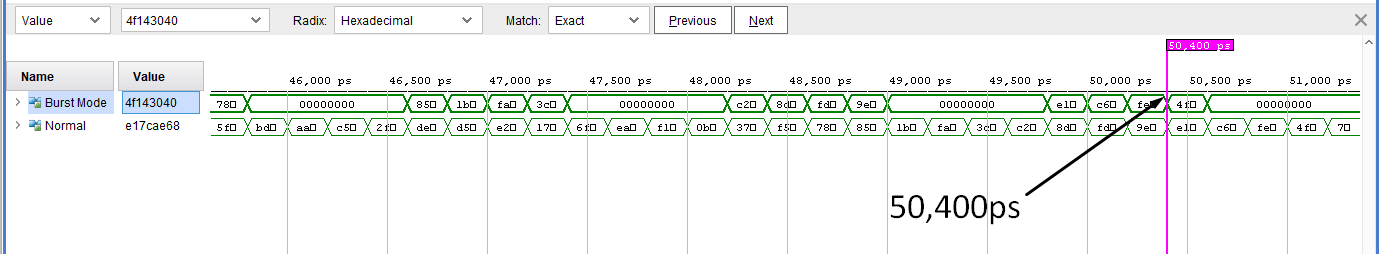
\includegraphics[width=1.5\linewidth]{img/burst_mode_3.png}
    \caption{Burst Mode Recur Time}%
    \label{fig:burst_mode_recur}
\end{figure}

\subsubsection{Switching Between Two Channels}%
\label{ssub:switching_between_two_channels}
Here the PRBS wrapper was changed to feed the two different outputs. The PRBS
generator was unchanged. We added a register which on overflow alternated the
output of the generator module. 
This had the overall effect of having the whole sequence be sent over two
different channels as shown in Figure~\ref{fig:two_channel_tx}.

\begin{figure}[ht]
    \centering
    \hspace*{-3cm}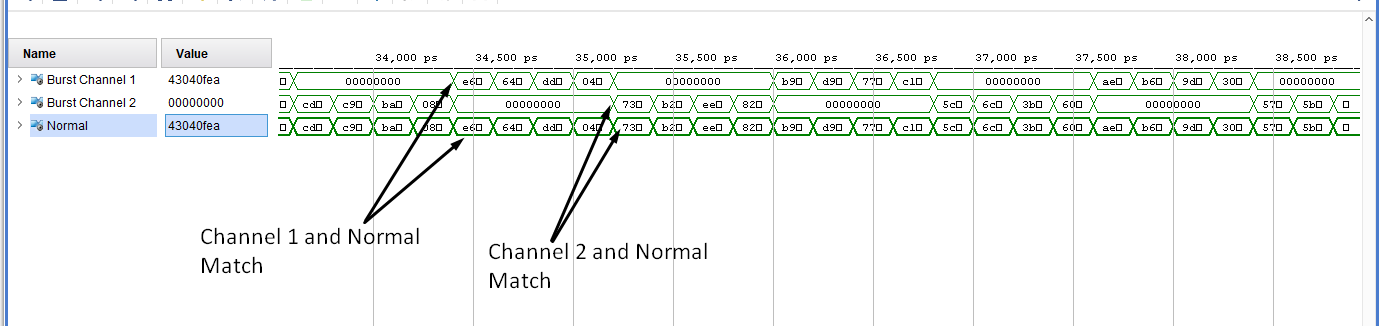
\includegraphics[width=1.4\linewidth]{img/two_channel.png}
    \caption{Two Channel Burst Mode}%
    \label{fig:two_channel_tx}
\end{figure}

\subsection{Reception}%
\label{sub:reception}
In Figure~\ref{fig:receiver_block} we see a block diagram of the receiver
(RX) of the transceiver. Serial data flows into the reciever, is deserialised,
and is finally passed to the RX Interface where it can then be passed to the
rest of the board.
\begin{figure}[ht]
    \centering
    \hspace*{-1cm}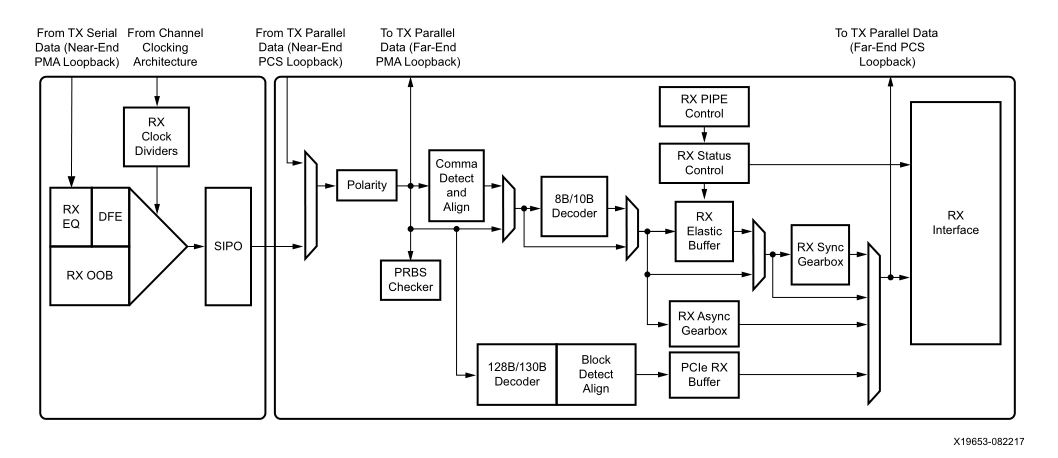
\includegraphics[width=1.2\linewidth]{img/receiver_block.png}
    \caption{Receiver Block Diagram \cite{GTY_guide}}%
    \label{fig:receiver_block}
\end{figure}

\subsubsection{Burst Mode Checking}%
\label{ssub:burst_mode_checking}
For burst mode checking there are some issues as there are periods when the
incoming bitstream is all zeros. The PRBS checker module takes the incoming
data as a seed to calculate the next expected sequence. If zeros are provided
then this interferes with the module (as the next expected word will be calculated
based on zeros). To compensate for this we added a register to the wrapper that
would not pass zeros to the checker module. 
In simulation when the PRBS generation module was connected directly to the
PRBS checker this worked correctly as shown in Figure~\ref{fig:burst_check_1}
with no errors thrown (the sequence was repeated nearly 4,000 times). 
\begin{figure}[ht]
    \centering
    \hspace*{-3cm}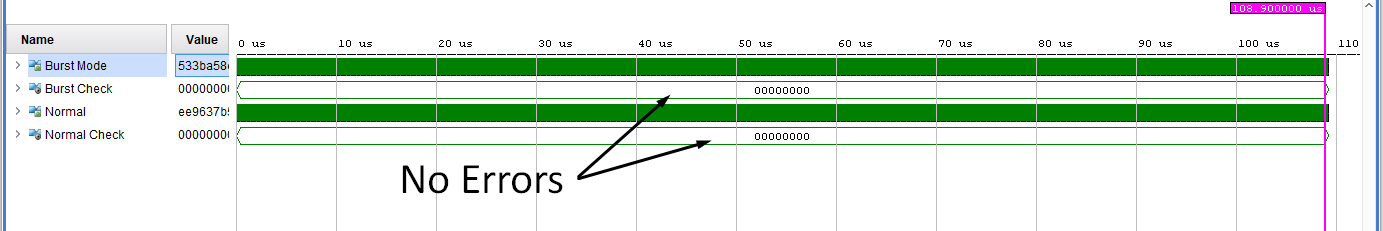
\includegraphics[width=1.5\linewidth]{img/burst_check.png}
    \caption{Direct Connection Checking}%
    \label{fig:burst_check_1}
\end{figure}

However, when passed through the transceiver, the PRBS checker found errors
consistently, as shown in Figure~\ref{fig:burst_check_2}. 
These errors appear to originate because in some situations where zeros are sent
to the TX interface, we recieve some bits at the RX interface. 
We suspect that this may be due to some encoding that the transceiver may be
doing, but were unable to pinpoint the cause.

\begin{figure}[ht]
    \centering
    \hspace*{-3cm}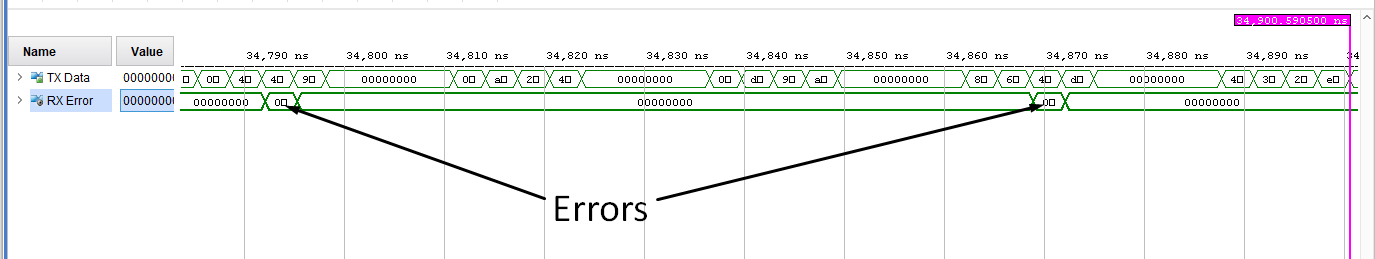
\includegraphics[width=1.5\linewidth]{img/burst_check_2.png}
    \caption{Transceiver Checking}%
    \label{fig:burst_check_2}
\end{figure}

\subsubsection{Two Channel Checking}%
\label{ssub:two_channel_checking}
In the case where two transmitters were muxed together and were sent to a
single receiver, it should not have been necessary to change the behaviour of
the PRBS checking module.
We were unable to experiment with this due to the closing of the lab.

\subsubsection{Disabling The CDR}%
\label{ssub:disabling_the_cdr}
The receiver CDR block detailed block diagram is shown in
Figure~\ref{fig:cdr_detail}.

\begin{figure}[ht]
    \centering
    \hspace*{-1cm}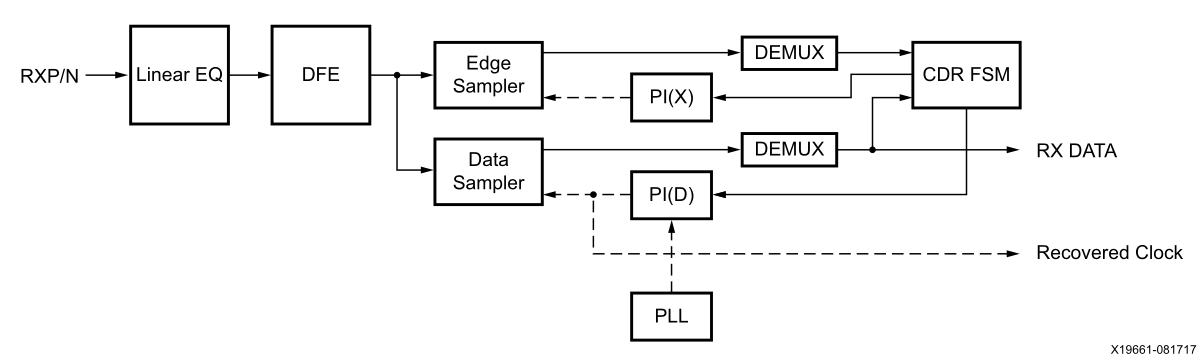
\includegraphics[width=1.2\linewidth]{img/cdr_detail}
    \caption{CDR Block Diagram}%
    \label{fig:cdr_detail}
\end{figure}

The final step would have been to run the receiver source-synchronously.  The
transceiver did not allow much flexibilty here. We attemped to do this was by
disabling the CDR and using the same clock to drive the reciever and
transmitter, ideally then we take readings of phase, and then make the
necessary compensations.
 
We were able to disable the CDR by asserting the CDRHOLD ports. This was done
by hardcoding the CDRHOLD value. We further extended this by adding CDRHOLD
in conjuction with the QPLLLOCK and RXCDRLOCK ports to the Xilinx Virtual
Input/Output (VIO) which allowed us to toggle the CDR.

The link became unstable after the port was asserted.  

We were then unable to read the phase. The phase caching paper by Kari, et al.
\cite{kari_phase} was done on Xilinx Ultra-scale board and they were able to
read and modify the phase by reading/writing values to the appropriate register.
However the details of that implementation were specific to the Ultra-scale
boards. The board used in the project is an Ultra-scale+ board and there is no
publicly available information on how to modify/read the phase. 
As such we were unable to explore this further.

\section{Optical Transmission}%
\label{optical_transmission}
This part of the project was not completed as the labs were closed before we
were able to test it. However some hardware was prepared, and is described in
the following sections.

\subsection{SOA Board}%
\label{sub:soa_board}
4 PCBs were prepared. The design consisted of an Inphenix SOA mounted in the
center. The electrical component was provided a matched RF line, and the laser
was coupled into the sides. A d-type connecter was also provided so that the
SOA could be temperature controlled.


\subsection{Heatsink and Mount}%
\label{sub:heatsink_and_mount}
It was also necessary to attach a aluminium substrate underneath the PCB board
for heat dissipation. 





\chapter{Conclusion}


% This displays the bibliography for all cited external documents. All references have to be defined in the file references.bib and can then be cited from within this document.
\bibliographystyle{IEEEtran}
\bibliography{ref}

% This creates an appendix chapter, comment if not needed.
\appendix
\chapter{Transceiver Settings}%
\label{cha:transceiver_settings}



The configuration of the Transceiver Wizard can be found here.

\begin{figure}[ht]
    \centering
    \hspace*{-2cm}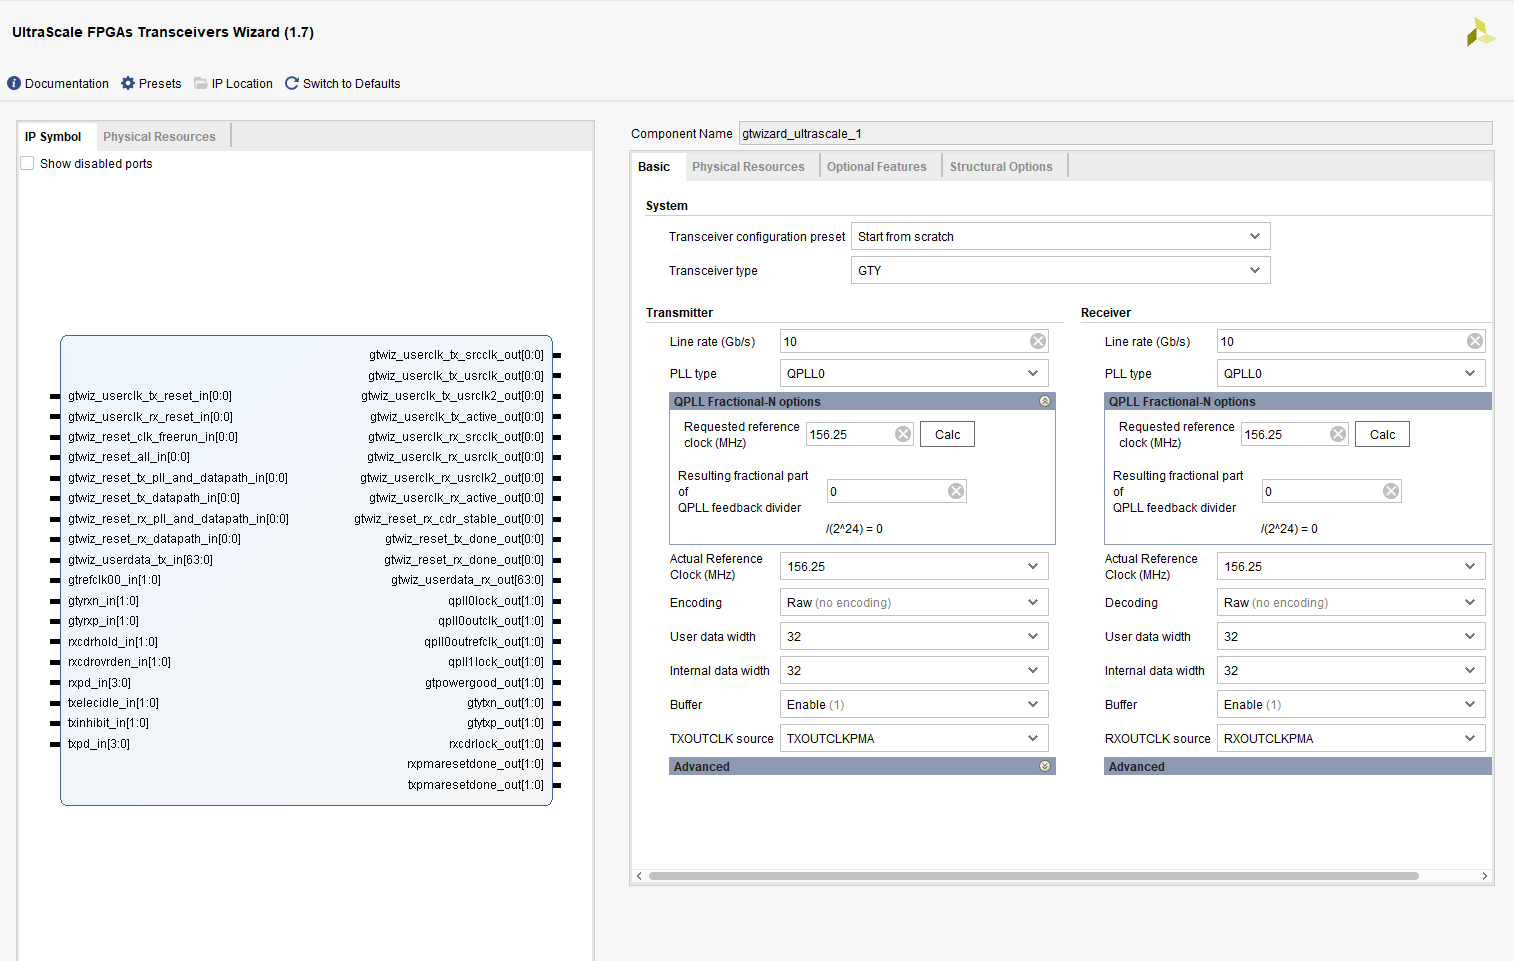
\includegraphics[width=1.3\linewidth]{img/transceiver1.png}
    \caption{Transceiver Wizard Settings}%
    \label{fig:transceiver1}
\end{figure}

\cleardoublepage

\begin{figure}[t]
    \centering
    \hspace*{-2cm}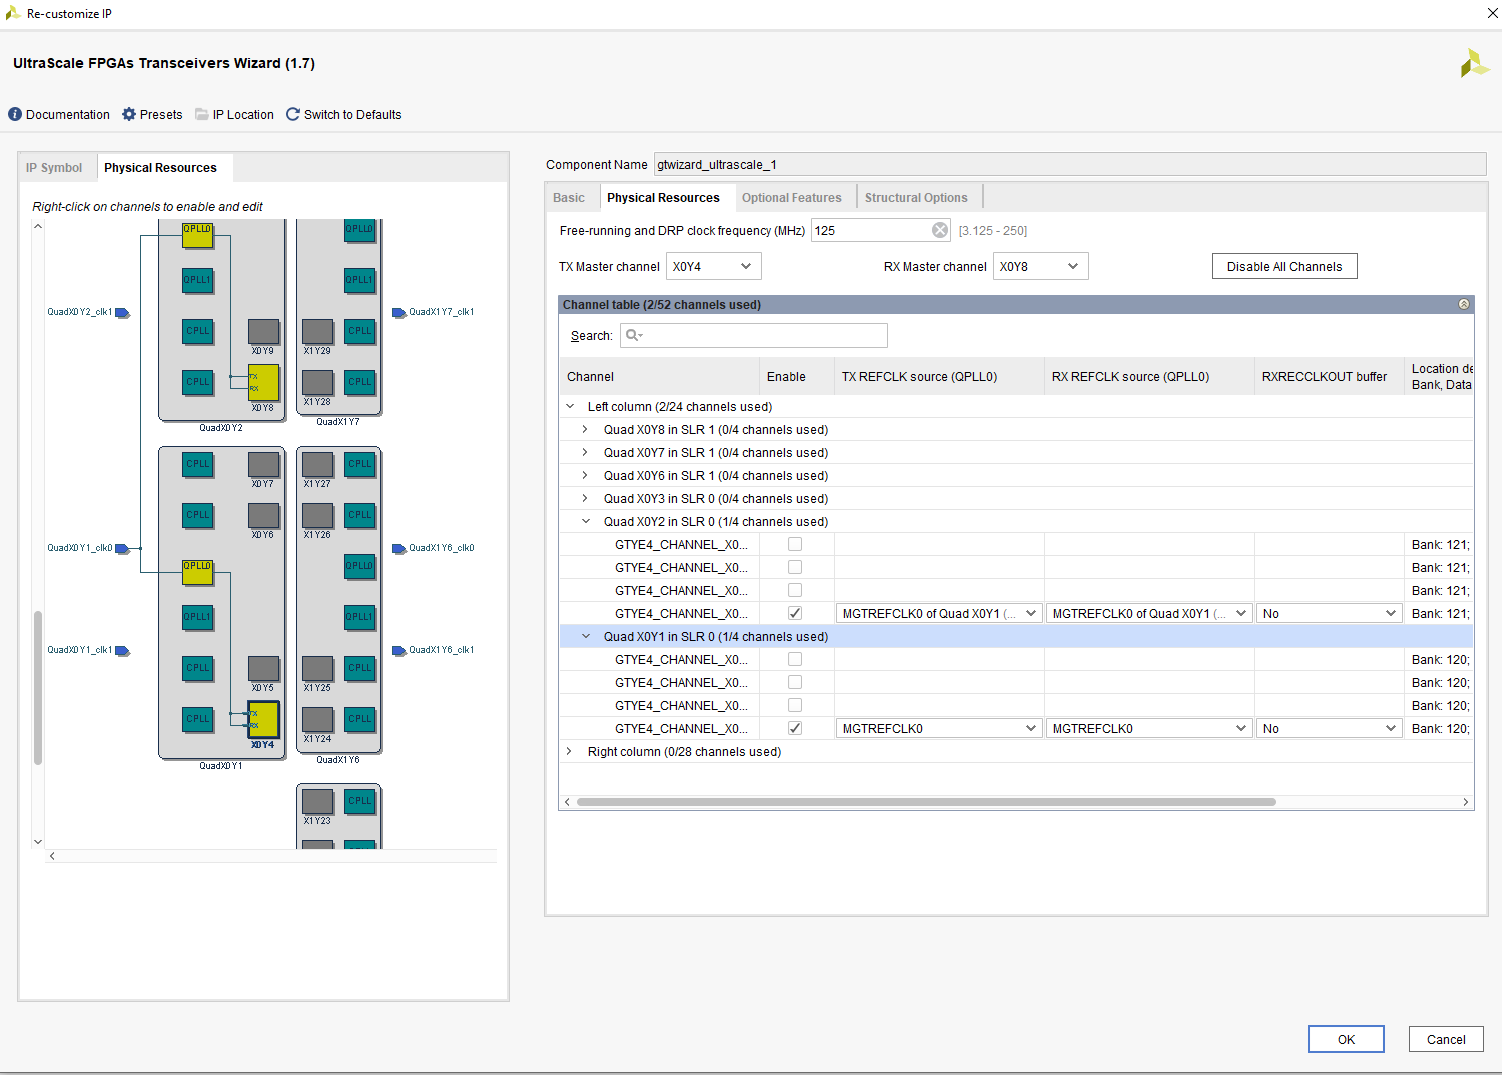
\includegraphics[width=1.3\linewidth]{img/transceiver2.png}
    \caption{Transceiver Wizard Settings 2}%
    \label{fig:transceiver2}
\end{figure}

\cleardoublepage

\begin{figure}[t]
    \centering
    \hspace*{-2cm}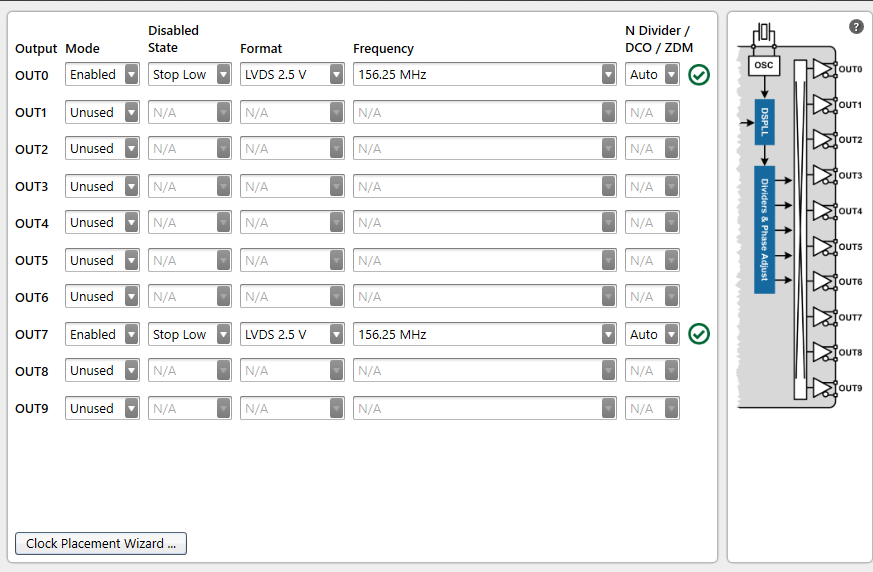
\includegraphics[width=1.3\linewidth]{img/clock_settings.png}
    \caption{External Clock Settings}%
    \label{fig:clock_settings}
\end{figure}

\cleardoublepage

\begin{listing}
\begin{minted}[linenos,numbersep=5pt,frame=lines,framesep=2mm]{c}

set_property PACKAGE_PIN AN41 [get_ports mgtrefclk0_x0y1_n] 
set_property PACKAGE_PIN AN40 [get_ports mgtrefclk0_x0y1_p]

set_property IOSTANDARD DIFF_SSTL12 [get_ports hb_gtwiz_reset_clk_freerun_in_p]

set_property PACKAGE_PIN AY23 [get_ports hb_gtwiz_reset_clk_freerun_in_n]
set_property PACKAGE_PIN AY24 [get_ports hb_gtwiz_reset_clk_freerun_in_p]
set_property IOSTANDARD DIFF_SSTL12 [get_ports hb_gtwiz_reset_clk_freerun_in_n]

set_property package_pin BE23 [get_ports hb_gtwiz_reset_all_in] 
set_property IOSTANDARD LVCMOS18 [get_ports hb_gtwiz_reset_all_in]

set_property PACKAGE_PIN BB24 [get_ports link_down_latched_reset_in]
set_property IOSTANDARD LVCMOS18 [get_ports link_down_latched_reset_in]


# LED1 (working correctly) 
set_property PACKAGE_PIN AV34 [get_ports link_status_out] 
set_property IOSTANDARD LVCMOS12 [get_ports link_status_out]

# LED0 (not working) 
set_property PACKAGE_PIN AT32 [get_ports link_down_latched_out] 
set_property IOSTANDARD LVCMOS12 [get_ports link_down_latched_out]

# Clock constraints for clocks provided as inputs to the core 
------------------------------------------------------------------------------
create_clock -period 8.000 -name clk_freerun [get_ports hb_gtwiz_reset_clk_freerun_in_p] 
create_clock -period 6.400 -name clk_mgtrefclk0_x0y1_p [get_ports mgtrefclk0_x0y1_p]

# False path constraints #
-------------------------------------------------------------------------------
set_false_path -to [get_cells -hierarchical -filter {NAME =~
*bit_synchronizer*inst/i_in_meta_reg}] 
set_false_path -to [get_cells -hierarchical -filter {NAME =~
*reset_synchronizer*inst/rst_in_*_reg}]
set_false_path -to [get_pins -filter REF_PIN_NAME=~*D -of_objects [get_cells
-hierarchical -filter {NAME =~ *reset_synchronizer*inst/rst_in_meta*}]]
set_false_path -to [get_pins -filter REF_PIN_NAME=~*PRE -of_objects [get_cells
-hierarchical -filter {NAME =~ *reset_synchronizer*inst/rst_in_meta*}]]
set_false_path -to [get_pins -filter REF_PIN_NAME=~*PRE -of_objects [get_cells
-hierarchical -filter {NAME =~ *reset_synchronizer*inst/rst_in_sync1*}]]
set_false_path -to [get_pins -filter REF_PIN_NAME=~*PRE -of_objects [get_cells
-hierarchical -filter {NAME =~ *reset_synchronizer*inst/rst_in_sync2*}]]
set_false_path -to [get_pins -filter REF_PIN_NAME=~*PRE -of_objects [get_cells
-hierarchical -filter {NAME =~ *reset_synchronizer*inst/rst_in_sync3*}]]
set_false_path -to [get_pins -filter REF_PIN_NAME=~*PRE -of_objects [get_cells
-hierarchical -filter {NAME =~ *reset_synchronizer*inst/rst_in_out*}]]


set_property C_CLK_INPUT_FREQ_HZ 300000000 [get_debug_cores dbg_hub]
set_property C_ENABLE_CLK_DIVIDER false [get_debug_cores dbg_hub] set_property
C_USER_SCAN_CHAIN 1 [get_debug_cores dbg_hub] connect_debug_port dbg_hub/clk
[get_nets hb_gtwiz_reset_clk_freerun_buf_int]
\end{minted}
\caption{Constraints}
\label{lst:constraints}
\end{listing}



\end{document}
